\section{Taxas uniformes e constante assintótica}
\label{sec:rates}

Para $f\in C^2[\alpha,\beta]$, use a extensão
\begin{equation}
F(x)=
\begin{cases}
f(\alpha)+f'(\alpha)(x-\alpha)+\tfrac12f''(\alpha)(x-\alpha)^2,&x<\alpha,\\
f(x),&\alpha\le x\le\beta,\\
f(\beta)+f'(\beta)(x-\beta)+\tfrac12f''(\beta)(x-\beta)^2,&x>\beta.
\end{cases}
\label{eq:c2-extension}
\end{equation}
Então $F\in C^2(\mathbb{R})$ e $\|F''\|_{\infty,\mathbb{R}}=\|f''\|_{\infty,[\alpha,\beta]}$. Seja $P_kF$ o interpolante nos nós $j2^{-k}$.

A fórmula local do resto da interpolação linear e a constante $1/8$ que dela
decorre são fatos clássicos da aproximação por splines
\citep{deboor2001,powell1981,schumaker2007}. A afirmação abaixo também prova o
limite uniforme e preserva a constante sob a racionalização específica da
biblioteca.

\begin{theorem}[cota aguda e limite]\label{thm:uniform}
Ponha $h=2^{-k}$ e $M=\|f''\|_{\infty,[\alpha,\beta]}$. Então
\begin{equation}
 \|f-P_kF\|_{\infty,[\alpha,\beta]}\le\frac{h^2M}{8},
 \label{eq:uniform-bound}
\end{equation}
e
\begin{equation}
 \lim_{k\to\infty}\frac{8}{h^2}\|f-P_kF\|_{\infty,[\alpha,\beta]}=M.
 \label{eq:uniform-limit}
\end{equation}
Além disso, para todo $\delta>0$ existe $g_{k,\delta}\in\Aclass([\alpha,\beta])$ com
\begin{equation}
 \|f-g_{k,\delta}\|_\infty\le\frac{h^2M}{8}+\delta.
 \label{eq:rational-rate}
\end{equation}
\end{theorem}

\begin{proof}
Em uma célula $[x_L,x_R]$ de largura $h$, ponha $e=F-P_kF$. Para $x\in(x_L,x_R)$, a função
\[
 \psi(t)=e(t)-\frac{(t-x_L)(t-x_R)}{(x-x_L)(x-x_R)}e(x)
\]
anula-se em $x_L,x,x_R$. Três aplicações de Rolle produzem $\xi_x\in(x_L,x_R)$ com $\psi''(\xi_x)=0$; portanto
\begin{equation}
 F(x)-P_kF(x)=\frac12F''(\xi_x)(x-x_L)(x-x_R).
 \label{eq:interpolation-remainder}
\end{equation}
O módulo do produto é no máximo $h^2/4$, com igualdade no centro, o que prova \eqref{eq:uniform-bound}.

Se $M=0$, \eqref{eq:uniform-limit} é imediata. Se $M>0$, escolha $x_*\in[\alpha,\beta]$ com $|f''(x_*)|=M$. Para cada $k$ suficientemente grande, escolha um centro de escala $k$, $z_k\in[\alpha,\beta]$, com $z_k\to x_*$. Avaliando \eqref{eq:interpolation-remainder} em $z_k$,
\[
 |F(z_k)-P_kF(z_k)|=\frac{h^2}{8}|F''(\xi_k)|,
\]
onde $\xi_k$ pertence à célula de $z_k$. O diâmetro da célula tende a zero, logo $\xi_k\to x_*$ e $|F''(\xi_k)|\to M$. Isso dá o limite inferior; \eqref{eq:uniform-bound} fornece o superior.

Para a última afirmação, racionalize todos os valores nodais da cobertura finita com erro menor que $\delta$ e mantenha valores adjacentes distintos, como no \cref{thm:density}. O interpolante resultante é uma montagem e dista menos que $\delta$ de $P_kF$ em norma uniforme. A desigualdade triangular conclui.
\end{proof}

\begin{corollary}[preservação da constante]\label{cor:rational-sharp}
Existe uma sequência $g_k\in\Aclass([\alpha,\beta])$ tal que
\[
 \lim_{k\to\infty}\frac{8}{h^2}\|f-g_k\|_\infty=M.
\]
\end{corollary}

\begin{proof}
Na construção do \cref{thm:uniform}, escolha erros nodais $\delta_k=o(h^2)$. Então
\[
 \bigl|\|f-g_k\|_\infty-\|f-P_kF\|_\infty\bigr|
 \le\|g_k-P_kF\|_\infty<\delta_k.
\]
Divida por $h^2/8$ e aplique \eqref{eq:uniform-limit}.
\end{proof}

Com $N_k$ de \eqref{eq:cell-count}, $h=(\beta-\alpha)N_k^{-1}(1+O(N_k^{-1}))$ e, portanto,
\begin{equation}
 \|f-P_kF\|_\infty
 \le \frac{(\beta-\alpha)^2M}{8}N_k^{-2}\bigl(1+O(N_k^{-1})\bigr).
 \label{eq:n-rate}
\end{equation}
Quando os extremos já são nós da malha, o termo de borda desaparece.

A \cref{tab:exp-pt} registra os valores exatos para $e^x$, enquanto a
\cref{fig:exp-pt} evidencia a convergência da razão para a constante aguda.

\begin{table}[t]
\centering
\caption{Erro exato do interpolante de $e^x$ em $[0,1]$.}
\label{tab:exp-pt}
\begin{tabular}{rrrr}
\toprule
$k$ & erro exato & $2^{-2k}e/8$ & razão\\
\midrule
2  & $1{,}8774\times10^{-2}$ & $2{,}1237\times10^{-2}$ & $0{,}8840$\\
4  & $1{,}2866\times10^{-3}$ & $1{,}3273\times10^{-3}$ & $0{,}9693$\\
6  & $8{,}2310\times10^{-5}$ & $8{,}2955\times10^{-5}$ & $0{,}9922$\\
8  & $5{,}1746\times10^{-6}$ & $5{,}1847\times10^{-6}$ & $0{,}9980$\\
10 & $3{,}2389\times10^{-7}$ & $3{,}2404\times10^{-7}$ & $0{,}9995$\\
\bottomrule
\end{tabular}
\end{table}

\begin{figure}[t]
 \centering
 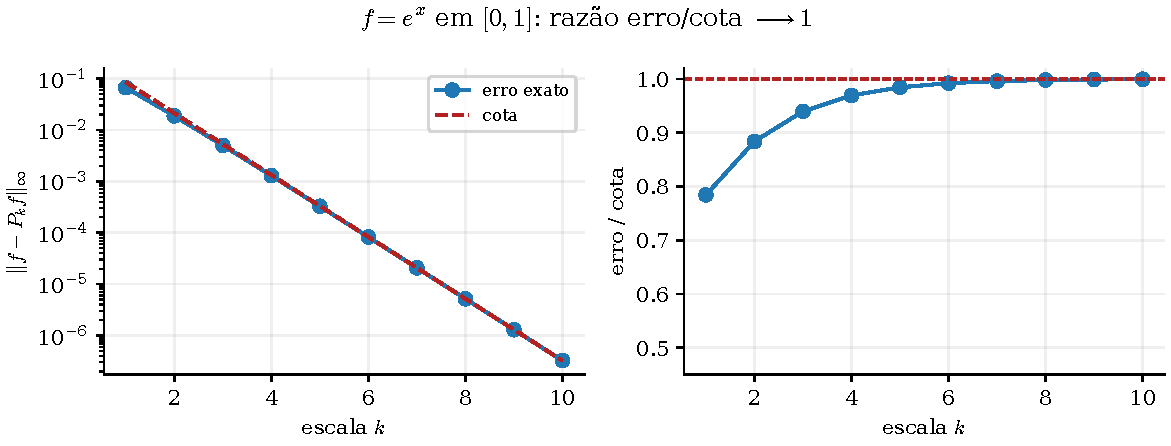
\includegraphics[width=.92\linewidth]{fig04_exp.pdf}
 \caption{A razão entre o erro exato e a cota converge a $1$, em concordância com \eqref{eq:uniform-limit}.}
 \label{fig:exp-pt}
\end{figure}
